
\begin{enumerate}
\item Si on choisit 8 comme nombre de départ, le programme donne 12 comme résultat.
\begin{center}
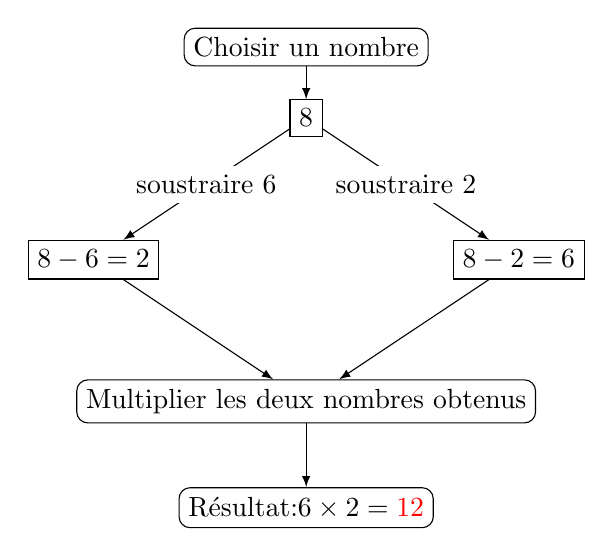
\begin{tikzpicture}[scale=.9]
\tikzstyle{rect}=[rectangle,draw]
\tikzstyle{ell}=[rectangle,rounded corners,draw]
\tikzstyle{fleche}=[->,>=latex]
\node[ell] (D) at (0,3) {Choisir un nombre};
\node[rect] (N) at (0,2) {$8$};
\node[rect] (S6) at (-3,0) {$8-6=2$};
\node[rect] (S2) at (3,0) {$8-2=6$};
\node[ell] (M) at (0,-2) {Multiplier les deux nombres obtenus};
\node[ell] (R) at (0,-3.5) {Résultat:$6\times 2=\textcolor{red}{12}$};
\draw[fleche] (D)--(N);
\draw[fleche] (N)--(S6) node[midway,fill=white] {soustraire 6};
\draw[fleche] (N)--(S2) node[midway,fill=white] {soustraire 2};
\draw[fleche] (S6)--(M);
\draw[fleche] (S2)--(M);
\draw[fleche] (M)--(R);
\end{tikzpicture}
\end{center}

\item Pour chacune des affirmations suivantes, indiquer si elle est vraie ou fausse. On rappelle que les réponses doivent être justifiées.
\begin{description}
\item[Proposition 1: VRAIE] Le programme peut donner un résultat négatif:
\begin{center}
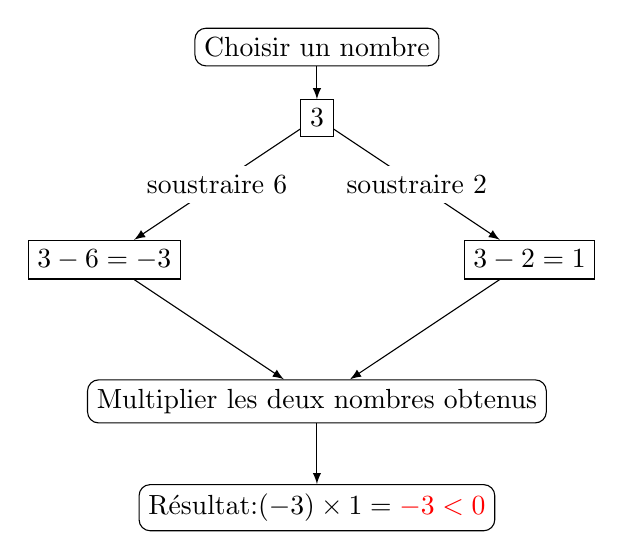
\begin{tikzpicture}[scale=.9]
\tikzstyle{rect}=[rectangle,draw]
\tikzstyle{ell}=[rectangle,rounded corners,draw]
\tikzstyle{fleche}=[->,>=latex]
\node[ell] (D) at (0,3) {Choisir un nombre};
\node[rect] (N) at (0,2) {$3$};
\node[rect] (S6) at (-3,0) {$3-6=-3$};
\node[rect] (S2) at (3,0) {$3-2=1$};
\node[ell] (M) at (0,-2) {Multiplier les deux nombres obtenus};
\node[ell] (R) at (0,-3.5) {Résultat:$(-3)\times 1=\textcolor{red}{-3<0}$};
\draw[fleche] (D)--(N);
\draw[fleche] (N)--(S6) node[midway,fill=white] {soustraire 6};
\draw[fleche] (N)--(S2) node[midway,fill=white] {soustraire 2};
\draw[fleche] (S6)--(M);
\draw[fleche] (S2)--(M);
\draw[fleche] (M)--(R);
\end{tikzpicture}
\end{center}


\item[Proposition 2: VRAIE] si on choisit $\dfrac{1}{2}$ comme nombre de départ, le programme donne $\dfrac{33}{4}$ comme résultat:
\begin{center}
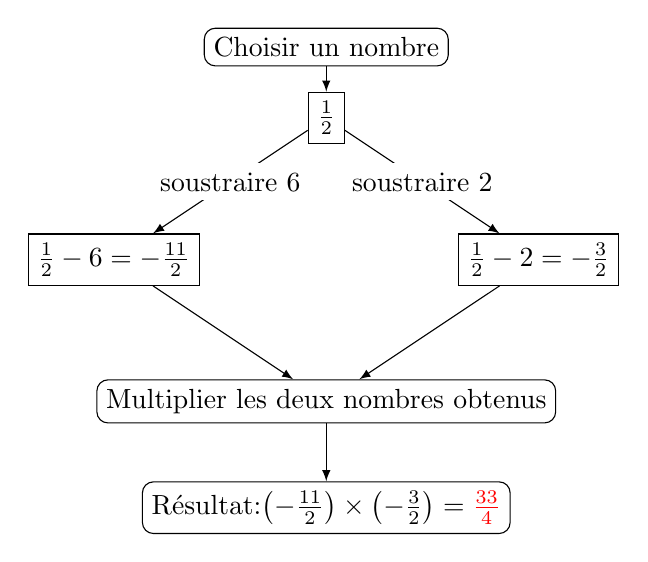
\begin{tikzpicture}[scale=.9]
\tikzstyle{rect}=[rectangle,draw]
\tikzstyle{ell}=[rectangle,rounded corners,draw]
\tikzstyle{fleche}=[->,>=latex]
\node[ell] (D) at (0,3) {Choisir un nombre};
\node[rect] (N) at (0,2) {$\frac{1}{2}$};
\node[rect] (S6) at (-3,0) {$\frac{1}{2}-6=-\frac{11}{2}$};
\node[rect] (S2) at (3,0) {$\frac{1}{2}-2=-\frac{3}{2}$};
\node[ell] (M) at (0,-2) {Multiplier les deux nombres obtenus};
\node[ell] (R) at (0,-3.5) {Résultat:$\left(-\frac{11}{2}\right)\times\left( -\frac{3}{2}\right)=\textcolor{red}{\frac{33}{4}}$};
\draw[fleche] (D)--(N);
\draw[fleche] (N)--(S6) node[midway,fill=white] {soustraire 6};
\draw[fleche] (N)--(S2) node[midway,fill=white] {soustraire 2};
\draw[fleche] (S6)--(M);
\draw[fleche] (S2)--(M);
\draw[fleche] (M)--(R);
\end{tikzpicture}
\end{center}

\vspace{0,5cm}

\item[Proposition 3: VRAIE] Le programme donne 0 comme résultat pour exactement deux nombres;
\begin{center}
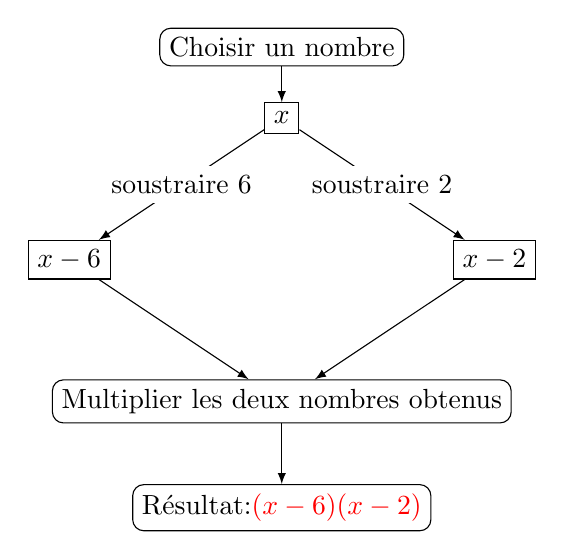
\begin{tikzpicture}[scale=.9]
\tikzstyle{rect}=[rectangle,draw]
\tikzstyle{ell}=[rectangle,rounded corners,draw]
\tikzstyle{fleche}=[->,>=latex]
\node[ell] (D) at (0,3) {Choisir un nombre};
\node[rect] (N) at (0,2) {$x$};
\node[rect] (S6) at (-3,0) {$x-6$};
\node[rect] (S2) at (3,0) {$x-2$};
\node[ell] (M) at (0,-2) {Multiplier les deux nombres obtenus};
\node[ell] (R) at (0,-3.5) {Résultat:\textcolor{red}{$(x-6)(x-2)$}};
\draw[fleche] (D)--(N);
\draw[fleche] (N)--(S6) node[midway,fill=white] {soustraire 6};
\draw[fleche] (N)--(S2) node[midway,fill=white] {soustraire 2};
\draw[fleche] (S6)--(M);
\draw[fleche] (S2)--(M);
\draw[fleche] (M)--(R);
\end{tikzpicture}
\end{center}
Ainsi, le résultat est nul si et seulement si (\textit{un produit est nul si et seulement si l'un des termes du produit est nul}):
\[
(x-6)(x-2)=0\Longleftrightarrow
\left\lbrace\begin{array}{c}
x-6=0\\
x-2=0
\end{array}\right.\Longleftrightarrow
\left\lbrace\begin{array}{c}
x=6\\
x=2
\end{array}\right.
\]
\item[Proposition 4: FAUX] la fonction qui, au nombre de départ, associe le résultat du programme est la fonction: $x\to .(x-6)(x-2)=x^2-8x+12$. Elle n'est pas de la forme $x\to ax$, donc non linéaire.
\end{description}
\end{enumerate}

\vspace{0,5cm}

